\subsection{Darfur is Dying}\subparagraph{URL}\url{http://www.darfurisdying.com/}\subparagraph{Description}Darfur is Dying, developed by mtvU, is a activism game released in April of 2006. The game consists of two main sections. In the first section, players must select a member of a Darfuri refugee; the family consists of a male, female, and several children. Once the player has chosen, the player must guide the refugee to a well using only compass and distance directions, while attempting to avoid Janjaweed militia patrols in trucks. If the player is caught, the game describes the fate of the refugee, and the player is prompted to select another refugee. Once the player has made it to the well, the player must return through the same section to their encampment, but lose water during their journey. Once they have returned to the encampment, the player enters a top-down strategy-like game simulation; they can use the water they have retrieved to grow crops and keep the encampment in good condition. However, if they run out of water, they will need to return to the first section and make the well run again. The goal of the game is to keep the encampment alive for 7 days. In addition, the community is constantly under threat from attacks from the militia; if the militia attacks, the encampment is lost, and the player must start again. The player can prevent attacks from the militia by participating in various viral and advocacy campaign tactics, such as inviting their friends to play, posting on social media, or writing to government officials.\subparagraph{Educational Content}The educational content of Darfur is Dying is centered almost entirely around awareness. Through playing the game, players learn about the nation of Darfur, including its history, wars, environment, climate, and people. The players are forced to be aware of the troubles that plight Darfuri residents and families, such as militia attacks. Players are encouraged to read the backstories of every man, woman, and child, as well as stories associated with locations within the village that expose various events that have happened, such as being unable to fend off sickness without medical aid, or when a militia recently stormed the village and murdered numerous people.\subparagraph{Notes on Implementation}Darfur is Dying was built in Flash by interactive media agency interFUEL.\begin{figure}[p]\centering 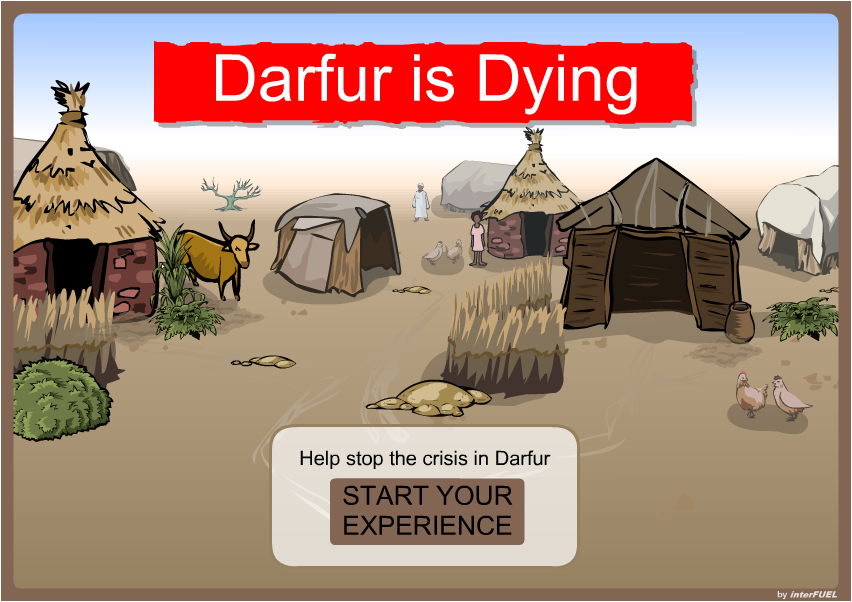
\includegraphics[height=.4\textheight, width=\textwidth, keepaspectratio=true]{img/darfur_title.png}\caption{Darfur is Dying's title screen}\end{figure}\begin{figure}[p]\centering 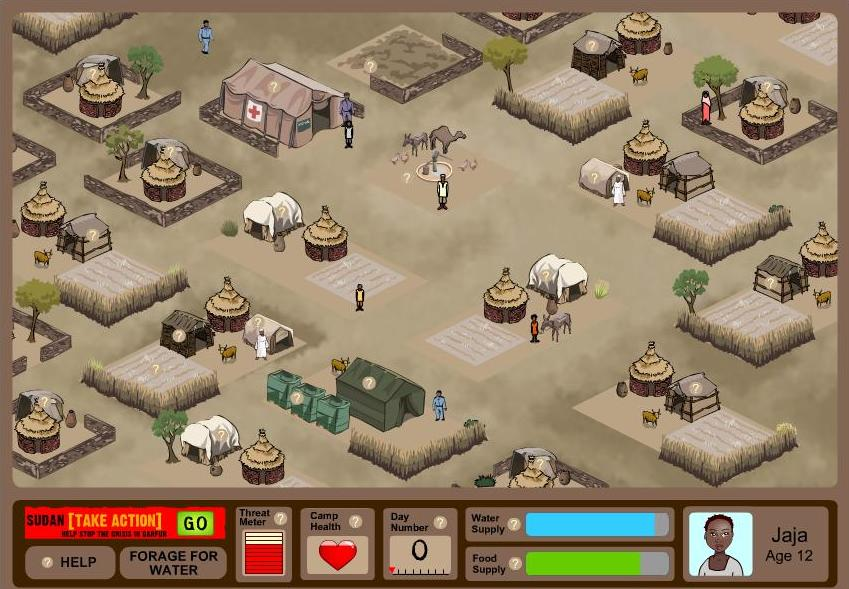
\includegraphics[height=.4\textheight, width=\textwidth, keepaspectratio=true]{img/darfur_screen1.jpg}\caption{A screenshot from Darfur Is Dying's village management section}\end{figure}\subsection{Light Bot}\subparagraph{URL}\url{http://armorgames.com/play/2205/light-bot}\subparagraph{Description}Light Bot, made by Danny Yaroslavski, is a programming and robotics puzzle game. It was originally a flash game, but has since been ported to iOS and Android. Players assume control of a robot on a grid of varying sizes and orientations. Each grid square can also have a height. The robot has the ability to move forward, turn left or right, jump up one level or down one level, and turn a square ``on." The robot also has the ability to call ``functions," where the robot can execute sequences of events and repeat functions several times or indefinitely. The goal of the robot is to navigate to all of the blue squares and turn them ``on" to a yellow state. The robot can do this in any order and using any sequence they like, so long as it fits within the provided instruction spaces. There are 40 levels to the game, ranging from the simple to extremely difficult.\subparagraph{Educational Content}Light Bot's educational purpose focuses on teaching programming at a very simple level. Players learn that the bot will follow sets of instructions. Initially, these instructions will be very simple (e.g. forward, turn, blink), but the player will realize quickly that the bot will follow the instructions explicitly, even if they do not solve the puzzle. This teaches players that computers are very powerful but very simple machines, and will do exactly what they are directed to do, even if it's not what the programmer intends to do. The game also teaches the concepts of functions and loops; players can ``call" predefined functions numerous times, as well as have a function call itself to loop the function indefinitely. These programming concepts, while simple, are a wonderful introduction to programming for students. \subparagraph{Notes on Implementation}Light Bot was built in Flash by Danny Yaroslavski, and the iOS and Android versions were built using Haxe 3 and OpenFL.\begin{figure}[p]\centering 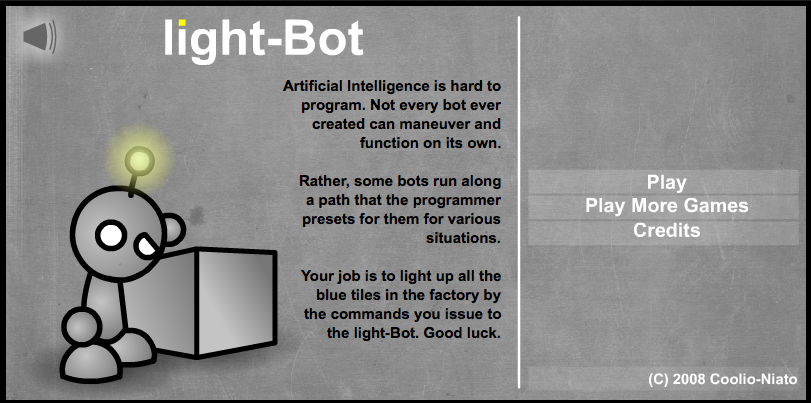
\includegraphics[height=.4\textheight, width=\textwidth, keepaspectratio=true]{img/lightbot_title.png}\caption{Light Bot's main menu}\end{figure}\begin{figure}[p]\centering 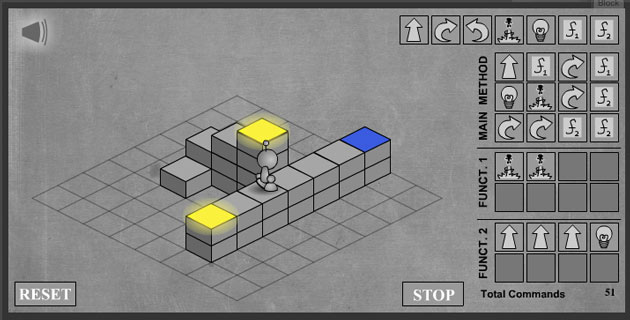
\includegraphics[height=.4\textheight, width=\textwidth, keepaspectratio=true]{img/lightbot_screen.jpg}\caption{A screenshot from one of Light Bot's levels}\end{figure}\subsection{Pandemic 2}\subparagraph{URL}\url{http://www.crazymonkeygames.com/Pandemic-2.html#game}\subparagraph{Description}Pandemic 2 is a flash-based strategy game involving infectious diseases, viruses, and bacteria. The player is in charge of designing and mutating an infectious organism, which infects the world population. The objective is to have the infection spread to and kill every human being on the planet, rendering the human race extinct. The virus starts out as being only mildly visible, lethal, and infectious, and can be mutated to more effective versions through ``upgrades," received as more humans are infected and die. To combat the spread of the infection, world nations begin to close their borders, set up quarantines, and close off trade routes, cutting off the transmission of the infection to their nation and making it more difficult or nearly impossible for the disease to spread. The player typically alters between the disease upgrade screen and the world monitoring screen, which includes notable headlines and the statuses of the nations. Global high scores are given to players that successfully eliminate the human race in the shortest amount of time.\subparagraph{Educational Content}Pandemic has two limited educational aspects to it. The first is the notion of learning about infectious diseases and organisms. While there isn't much science within the game behind mutating an organism to be more deadly, there are plenty of terms and game mechanics that the player can familiarize themselves with, such as organism's resistance to humidity, or how airborne diseases differ from waterborne. There's also an element of strategizing, risk-taking, and planning ahead associated with playing the game; if players run into a problem with a certain method, they may be able to solve the problem a different way, or circumvent the problem on another playthrough.\subparagraph{Notes on Implementation}Pandemic 2 was built in Flash by Dark Realm Studios.\begin{figure}[p]\centering 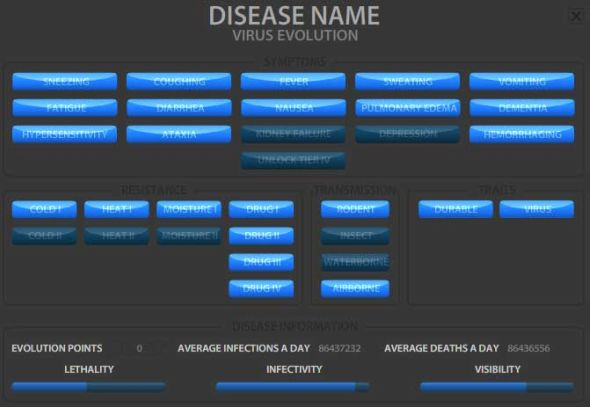
\includegraphics[height=.4\textheight, width=\textwidth, keepaspectratio=true]{img/pandemic_screen.jpg}\caption{A screenshot from Pandemic 2's evolution view}\end{figure}\subsection{Oregon Trail}\subparagraph{URL}\url{http://www.virtualapple.org/oregontraildisk.html}\subparagraph{Description}The Oregon Trail is a series of games detailing the experience of a pioneers traveling the Oregon Trail, a wagon route from the Missouri River to Oregon in 1848. The original game, developed for the HP 2100 in December of 1971, turned out to be extremely well received by middle and high school students. In the game, the player first selects an identity which determines how much starting money they have. They then select supplies to buy for their journey; wagons, spare parts, oxen, food, and other supplies. Once they embark on their journey, time passes and food is automatically consumed. Occasionally, players have the chance to hunt, where they can play a simple top-down 2D game to shoot animals that provide food to their party. In addition, numerous events will happen that the player needs to make descisions for, such as a party member falling ill, a wagon part breaking or oxen becoming injured, or needing to cross a river. The player's objective is to travel the entire Oregon Trail with using the minimum amount of resources; the player receives more points at the end for having living party members, items in inventory, and number of dollars, as well as receiving a multiplier if they started the game with less cash.\subparagraph{Educational Content}Oregon Trail's educational value comes in two forms. The first is the most apparent one; though not explicitly sitting players down and teaching them, the game educates students on life in the 19th century, as well as the hardships and trials endured by explorers of the early Oregon Trail. It teaches them about the kinds of materials that were used in everyday life, like wagons and oxen, as well as the diseases that commonly plagued explorers (diarrhea, dysentery), and what day-to-day activities were like on the trails, such as maintaining the wagons, crossing rivers, and hunting for food. The other educational aspect that Oregon Trail focuses on is planning and risk management; though not explicitly teaching players how to assess the risk of various actions, players who properly evaluate their initial inventory options as well as the options they have during events on the trail will end up doing better than players who don't.\subparagraph{Notes on Implementation}This is the very first edition of The Oregon Trail, for the Apple II. It's played in a browser-based Apple II emulator.\begin{figure}[p]\centering 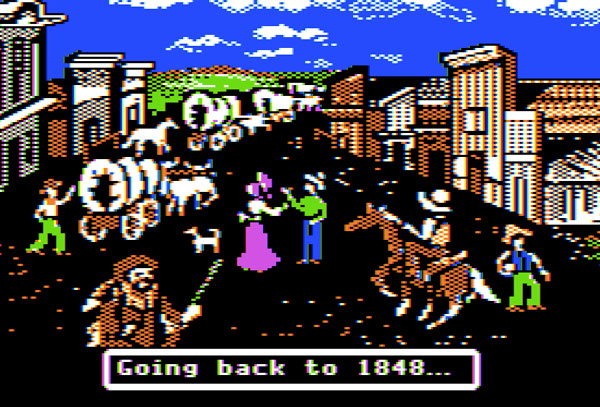
\includegraphics[height=.4\textheight, width=\textwidth, keepaspectratio=true]{img/oregon_title.jpg}\caption{A screenshot from the opening sequence of Oregon Trail}\end{figure}\begin{figure}[p]\centering 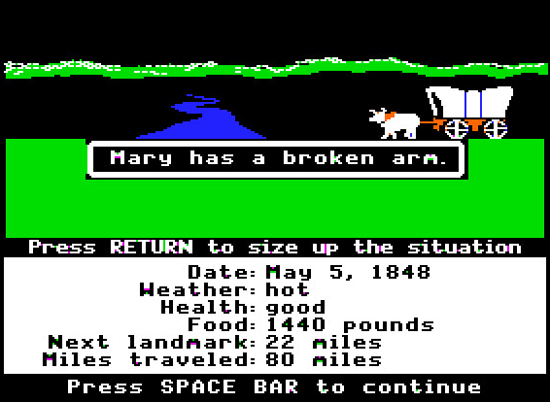
\includegraphics[height=.4\textheight, width=\textwidth, keepaspectratio=true]{img/oregon_screen.jpg}\caption{A screenshot from the gameplay of Oregon Trail}\end{figure}\subsection{Number Munchers}\subparagraph{URL}\url{http://wallofgame.com/free-online-games/arcade/988/Number_Munchers.html}\subparagraph{Description}Number Munchers is part of a ``Munchers" series that began as a strictly educational game around teaching children basic arithmetic and other numerical concepts. The series then expanded to teach words and other knowledge. The player first selects the educational content that they'd like to play, including grade level. Administrative controls are available for parents and teachers to restrict what kind of content is available; for example, restricting higher-grade students to their level, instead of allowing them to play at trivial levels. Once in the game, the player assumes control of a green 'Muncher,' which can move up, down, left or right. The game board is a grid, with each space containing a number that is a solution to the level they're playing (e.g. equal to 12, multiples of 3, divisible by 5). The player moves onto the appropriate space, and presses the space key to 'eat' the number. If the number matches the level criteria, the player gets points; if it does not, the player loses one of three lives. The player also has to deal with 'troggles,' which cross the grid slowly at random intervals. If the player occupies the same space as a troggle, the player loses a life and is reset to a different grid space. The level ends once all the appropriate numbers are eaten, and the player recieves a bonus for time.\subparagraph{Educational Content}The educational content of Number Munchers is extremely straightforward. Players will learn arithmetic, primes, and other numerical concepts while playing this game. Players who learn the concepts will be able to identify the correct solutions faster, and consequently achieve a higher score while playing this game.\subparagraph{Notes on Implementation}This is not an official version of Number Munchers. It's a Flash-based, Number Munchers-inspired game created by user Authorblues. It's functionally equivalent to the original edition of Number Munchers.\begin{figure}[p]\centering 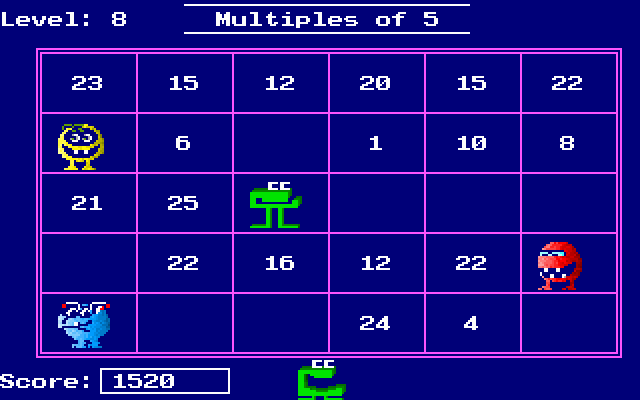
\includegraphics[height=.4\textheight, width=\textwidth, keepaspectratio=true]{img/munchers_screen.png}\caption{A screenshot from the gameplay of Number Munchers}\end{figure}\subsection{BotLogic}\subparagraph{URL}\url{http://botlogic.us/}\subparagraph{Description}BotLogic is an educational programming game. In the game, the players assume control of a robot whose task is to return home. The game takes place on a grid, with the robot located on one space, the home on another space some distance away, and a number of obstacles in between. The player can direct the robot up, down, left, or right, and does so by queueing up commands before running the program. The player can wait for the program to run, then add more commands before running the rest of the program, which allows players to incrementally build their program. However, the robot has a limited amount of energy, which limits the number of moves the player can take. Later in the game, more obstacles and powerups are introduced, such as electric fences, buttons, and recharging stations. The game contains 20 levels.\subparagraph{Educational Content}Botlogic teaches players about simple programming concepts, namely passing a sequence of instructions to a robot and watching them run. However, the game doesn't include any functional or object-oriented programming concepts, and is only slightly abstracted away from the player having direct directional control of the robot.\subparagraph{Notes on Implementation}BotLogic is built in HTML5/Javascript and developed by Dolphin Micro, a web development consulting firm located in Colorado.\begin{figure}[p]\centering 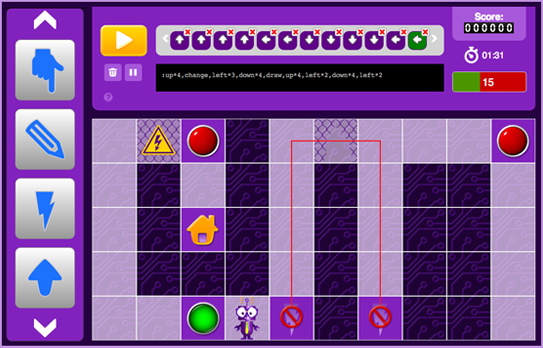
\includegraphics[height=.4\textheight, width=\textwidth, keepaspectratio=true]{img/botlogic_screen.png}\caption{One of the levels from BotLogic}\end{figure}\subsection{Math Baseball}\subparagraph{URL}\url{http://www.funbrain.com/math/index.html}\subparagraph{Description}Math Baseball is an educational math game. Initially, the player selects what type of arithmetic they'd like to do, as well as the grade level. Then, they assume the role of a baseball player at bat. For each throw, the players are given unlimited time to answer one arithmetic question. If they get the question right, the player earns a randomly selected single, double, or triple and gets a runner on base, as well as advancing any other runners. The player's score is determined by how many runs they get in. If they don't get the question right, then they recieve a strike. After three strikes, the player is ``out," and the game ends.\subparagraph{Educational Content}The education in ``Math Baseball" is very straightforward. Players can learn addition, subtraction, multiplication, and division, with the player's knowledge of the topic reflected in their higher score of the game.\subparagraph{Notes on Implementation}Math Baseball is written in HTML and an unspecified server framework.\begin{figure}[p]\centering 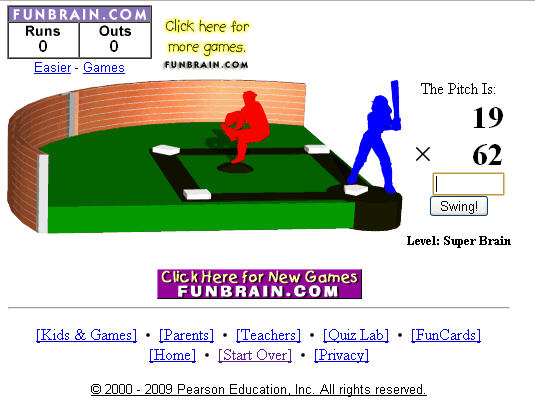
\includegraphics[height=.4\textheight, width=\textwidth, keepaspectratio=true]{img/baseball_screen.jpg}\caption{A screenshot from the gameplay of Math Baseball}\end{figure}\subsection{Notpron}\subparagraph{URL}\url{http://notpron.org/notpron/}\subparagraph{Description}Notpron is an ARG (alternate-reality game) for the browser. The player begins Level 1 with an image of a house with a partially open door in front, as well as some slightly opaque text that says ``Enter the door." The player needs to click the door (not the image, but the door itself) to advance to Level 2. In Level 2, a finger points to the address bar, where the player can replace ``level2.htm" with ``level3.htm" to advance to the next level. In Level 3, the player must change ``false" in the URL to ``true" to advance to the next level. The game continues like this, adding in new elements each level. There are a total of 140 levels, and only 31 people have completed all 140 levels, out of about 16 million players.\subparagraph{Educational Content}From the Notpron site: \quotation{``[Players who finish the game] have persisted with a broad range of complex ways of thinking, while maintaining focus and dedication over a long period. [Their] detective skills have been tested to the limits, yet the smallest hint proved sufficient to solve the most complicated tasks. Furthermore, competence in the following areas have been displayed: Sound editing, Graphic editing, Musical understanding, Insight into HTML programming, Rapid learning of new programs, Efficient online research techniques, [and] Insight into the complex workings of a computer."}\subparagraph{Notes on Implementation}Notpron is written in HTML and an unspecified server framework.\begin{figure}[p]\centering 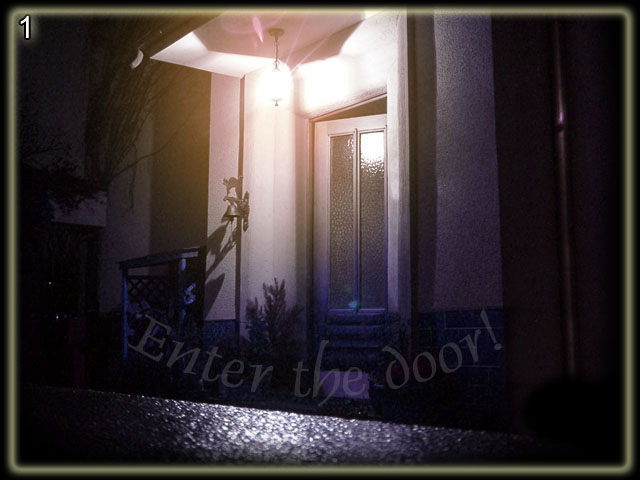
\includegraphics[height=.4\textheight, width=\textwidth, keepaspectratio=true]{img/notpron_screen.jpg}\caption{The first level of Notpron}\end{figure}\subsection{Lemmings}\subparagraph{URL}\url{http://www.elizium.nu/scripts/lemmings/}\subparagraph{Description}Lemmings, a PC game, was originally developed in 1991. The game plays from a 2D side-scrolling perspective. The player directs ``lemmings," small, humanoid creatures that are reminiscient of the mammal in their behavior. They operate almost entirely on their own, walking in one direction until they run into something, then reversing direction. They begin by dropping out of the entrance door, and successfully exit the level through another door in the level. However, the lemmings are very susceptible to dying; falling too far without a parachute will kill them, and numerous obstacles litter the courses, such as spike pits and smashers. The game contains four difficulty levels, with roughly 20 levels per difficulty level.\subparagraph{Educational Content}Lemmings teaches players problem-solving, multitasking, and resource management. Because a fixed number of lemmings are required to finish the level, players must learn the proper methods for getting around obstacles by using the minimum number of lemmings possible.\subparagraph{Notes on Implementation}This implementation of Lemmings is a Javascript port of the original version of the game.\begin{figure}[p]\centering 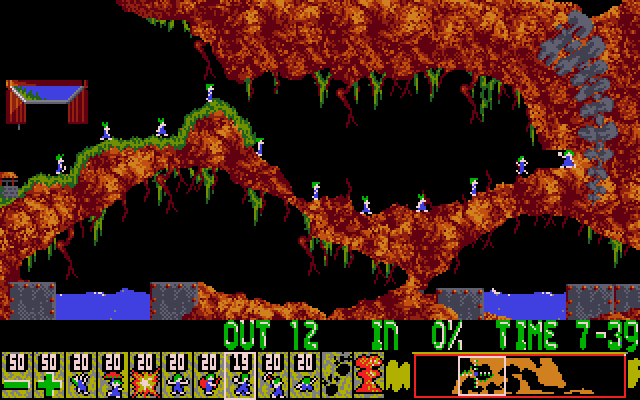
\includegraphics[height=.4\textheight, width=\textwidth, keepaspectratio=true]{img/lemmings_screen.jpg}\caption{One of the levels from Lemmings}\end{figure}\subsection{The Incredible Machine}\subparagraph{URL}\url{http://www.classicdosgames.com/online/timdemo.html}\subparagraph{Description}The Incredible Machine, originally developed in 1993, is a side-view 2D construction game. During a level, the player will have an objective (e.g. get the ball into the basket). The play area will already have some parts set up, so the player can use the parts that they have in reserve to construct the rest of the Rube Goldberg-style machine to accomplish the objective. There were around 80 levels in the game. The game was extremely successful, and spawned numerous sequels and ports.\subparagraph{Educational Content}The Incredible Machine teaches players about physics and problem solving. Players learn about the physical properties of various objects (for example, the tennis ball might not knock down the board, but the bowling ball might), and learn how to use limited combinations of those objects together to solve the puzzles. \subparagraph{Notes on Implementation}This is the original edition of The Incredible Machine, run inside a Java container in the browser.\begin{figure}[p]\centering 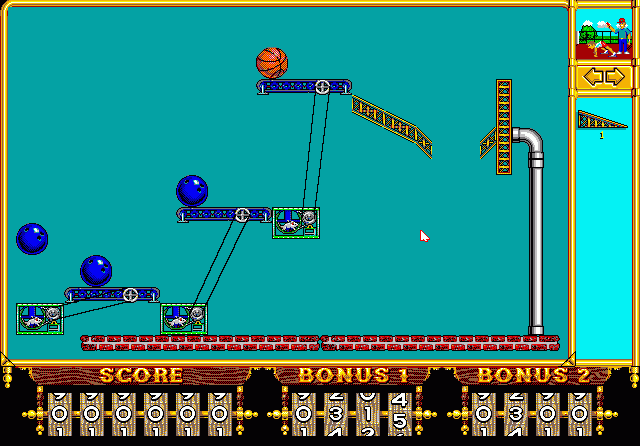
\includegraphics[height=.4\textheight, width=\textwidth, keepaspectratio=true]{img/machine_screen.png}\caption{One of the levels from The Incredible Machine}\end{figure}